%==========================================================================

\begin{frame}[fragile]

  {\Huge Tuning Changes Demo}

  \vspace{10pt}

\end{frame}

%==========================================================================

% Examples

% note: always keep the [fragile] for your frames!

\begin{frame}[fragile]{Kokkos Runtime Tuning Overview/Review (1/7)}
  \begin{itemize}
      \item Kokkos has runtime auto-tuning support when configured with
      \begin{itemize}
        \item \texttt{Kokkos\_ENABLE\_TUNING} CMake variable enabled at configuration time
      \end{itemize}
      \item Kokkos internal auto-tuning support is enabled at runtime when
      \begin{itemize}
        \item \texttt{--kokkos-tune-internals} command line variable enabled at run time
        \item a Kokkos tool is used to provide the search
      \end{itemize}
      \item Internal tunable parameters (available before 4.5)
      \begin{itemize}
        \item \texttt{MDRangePolicy} - $X$, $Y$, $Z$ block sizes for CUDA, HIP execution spaces
        \item \texttt{TeamPolicy} - team size and vector length for CUDA, HIP execution spaces
      \end{itemize}
      \item Arbitrary runtime parameters can be tuned with the same API, code modifications required - we hope to simplify (or abstract) that API
  \end{itemize}
\end{frame}

\begin{frame}[fragile]{Kokkos Runtime Tuning New Features (2/7)}
  \begin{itemize}
      \item New Internal tunable parameters (4.5)
      \begin{itemize}
        \item \texttt{RangePolicy} - Occupancy (with code modification) for CUDA execution space
        \item \texttt{MDRangePolicy} - Occupancy (with code modification) for CUDA execution space
        \item \texttt{TeamPolicy} - Occupancy (with code modification) for CUDA execution space
      \end{itemize}
      \item Occupancy value tuned between [5:100], step size of 5
      \item Natural extension of PR \#3379: ``Experimental feature: control cuda occupancy''
      \begin{block}{}
          \textit{``...passing \texttt{prefer(policy, DesiredOccupancy(33))} to a \texttt{parallel\_for()}, \texttt{parallel\_reduce()}, or \texttt{parallel\_scan} will bypass the block size deduction that tries to maximize the occupancy and adjust the launch parameters (by fixing the block size and requesting shared memory) to achieve the specified occupancy. The desired occupancy is in percent.''}
      \end{block}
  \end{itemize}
\end{frame}

\begin{frame}[fragile]{Occupancy Example - code change required (3/7)}
    \begin{code}[keywords={std}]
    using memory_space = typename Kokkos::DefaultExecutionSpace::memory_space;
    using view_type = Kokkos::View<double **, memory_space>;
    view_type left("process_this", 1000000, 25);
    /* Create a policy wrapper to request a tuned occupancy value from 0-100 */
    auto const occupancy_policy = Kokkos::Experimental::prefer(
        Kokkos::RangePolicy<>(0, left.extent(0)),
        Kokkos::Experimental::DesiredOccupancy{Kokkos::AUTO});
    const auto kernel = KOKKOS_LAMBDA(int i) {
            for (int r = 0; r < 25; r++) {
                double f = 0.;
                for (int m = 0; m < left.extent_int(1); m++) {
                    f += left(i, m);
                    left(i, m) += f;
                }
            }
        };
    Kokkos::parallel_for("Bench", occupancy_policy, kernel);
    \end{code}
\end{frame}

\begin{frame}[fragile]{APEX Auto-tuning Support (4/7)}
  \begin{itemize}
      \item APEX 2.7.0 released: \url{https://github.com/UO-OACISS/apex}
      \item Included as git submodule in kokkos-tools: \url{https://github.com/kokkos/kokkos-tools/tree/develop/tpls/apex}
      \item Profiling and tracing support for both asynchronous tasking runtimes and ``conventional'' parallel models (MPI, OpenMP, OpenACC, OpenCL, CUDA, HIP, SYCL, Kokkos, Pthreads, HPX, PaRSEC, StarPU, Iris...)
      \item Runtime adaptation search strategies (exhaustive, random, simulated annealing, genetic search, nelder mead, auto) integrated with Kokkos tuning API
      \item Growing set of example cases: \url{https://github.com/khuck/apex-kokkos-tuning}
      \item Long article on Kokkos autotuning with APEX: \url{https://github.com/UO-OACISS/apex/wiki/Kokkos-Runtime-Auto-Tuning-with-APEX}
  \end{itemize}
\end{frame}

\begin{frame}[fragile]{Running with APEX (5/7)}
    \begin{code}[keywords={bash}]
# Specify the search strategy
export APEX_KOKKOS_TUNING_POLICY=nelder_mead
# Specify the number of samples to be taken for each configuration
export APEX_KOKKOS_TUNING_WINDOW=4
# Run with apex_exec
apex_exec --apex:kokkos-tuning ./occupancy_example --kokkos-tune-internals

# Possible (truncated) verbose output:
...
Nelder Mead: New best! 0.00197833 k: 1, Bench: 30
Nelder Mead: New best! 0.00196357 k: 7, Bench: 20
Nelder Mead: New best! 0.00196042 k: 10, Bench: 25
Nelder Mead: New best! 0.00195894 k: 48, Bench: 25
...
Converged after 43 iterations.
Total func evaluations: 114
APEX: Tuning has converged for session 1.
[25]

    \end{code}
\end{frame}

\begin{frame}[fragile]{Perfetto trace of example tuned by APEX for Nelder Mead search strategy (6/7)}
    \begin{center}
    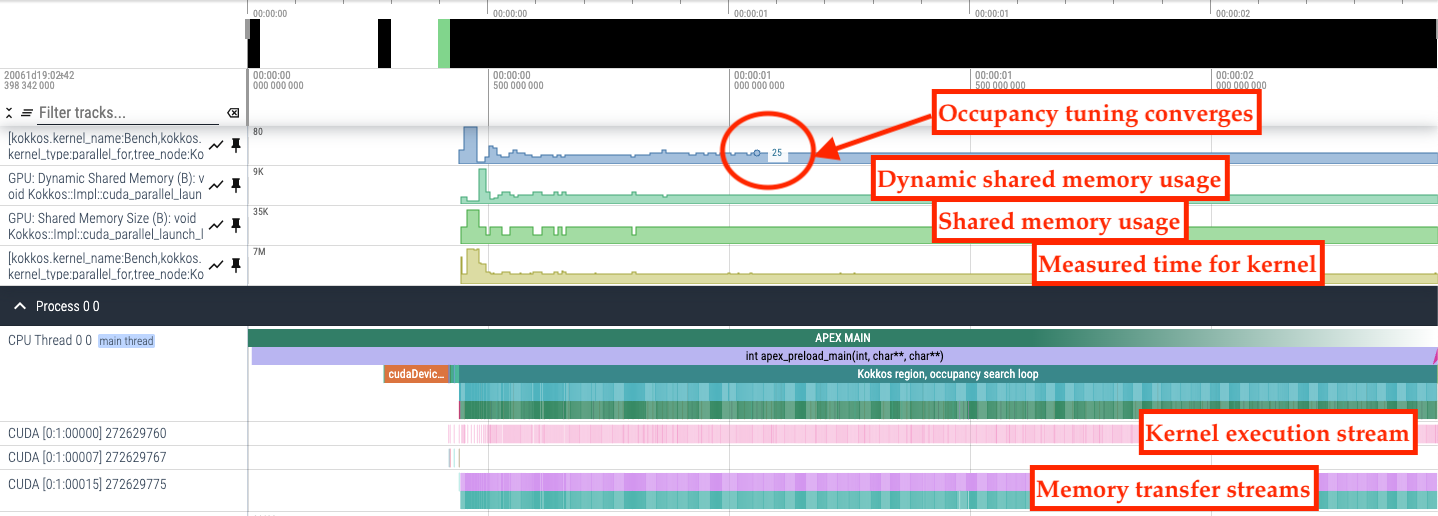
\includegraphics[width=\linewidth]{4_5/tuning/nelder_mead_occupancy_trace.png}
    \end{center}
\end{frame}

\begin{frame}[fragile]{Kokkos Potential Future Tuning Plans (7/7)}
  \begin{itemize}
      \item Simplified/abstracted API for custom tuning in user code (or at least some helper functions)
      \begin{itemize}
        \item \texttt{kokkosp\_declare\_[input,output]\_type} - make it easier to create variables
        \item \texttt{kokkosp\_[begin,end]\_context}
        \item \texttt{kokkosp\_request\_values}
      \end{itemize}
      \item Additional examples, performance studies
      \item Internal tuning for \texttt{RangePolicy}
      \item Internal support/testing for more execution engines (SYCL, OpenMP, OpenMPTarget)
  \end{itemize}
\end{frame}

%==========================================================================
